\section{Introducción}
\textit{Ruby on Rails} es un framework que hace facilita el desarrollo, la implementación, y el mantenimiento de aplicaciones web. Durante unos meses después de su lanzamiento incial, \textit{Rails} pasó de ser un ``juguete'' desconocido a ser un fenómeno mundial; y lo que es mucho más importante, se ha convertido en el framework más elegido para la implementación de muchísimas de las llamadas aplicaciones web 2.0.

La reputación de \textit{Ruby on Rails} es enorme debido a una serie de razones. Primero, un gran colectivo de desarrolladores estaban frustrados con tecnologías que ellos utilizaban para crear aplicaciones web. Sin importar si usaban \textit{Java}, \textit{PHP}, o .\textit{NET}, el sentimiento e idea general que tenía de su trabajo es que era demasiado difícil.

La sencillez no lo es todo. Los programadores profesionales, necesitaban la sensación de que las aplicaciones que desarrollaban aguantarían el paso del tiempo, implementado diseños y tecnologías modernas con técnicas profesionales. Naturalmente, estos desarrolladores miraron \textit{Rails} y descubrieron que era una herramienta muy potente para el desarrollo de aplicaciones web.

Un ejemplo de ello es, todas las aplicaciones de \textit{Rails} son implementadas usando la arquitectura modelo-vista-controlador (MVC). Los desarrolladores de \textit{Java} están habituados a frameworks como \textit{Taperstry} o \textit{Struts}, que están basados en MVC. Pero \textit{Rails} eleva la arquitectura MVC mucho más allá, cuando se desarrolla una aplicación en \textit{Rails}, se empieza con una aplicación que funciona desde el momento cero, y que todas las piezas del código interactuan las unas con las otras de una forma estándar.

Los desarrolladores se preocupan por la implantación del sistema también. Encontraron en \textit{Rails} una forma de implantar aplicaciones en cualquier número de servidores con un solo comando.\cite{RubyThomasHansson2013}

La última cosa a comentar respecto a este apartado es que Sam Ruby, Dave Thomas, David Heinemeier Hansson y otros muchos desarrolladores piensan que hay algo más sobre \textit{Ruby on Rails}, algo bastante difícil de explicar, la sensación de que se están haciendo las cosas bien y como es debido. Al igual que otros muchos, yo también creo lo mismo sobre \textit{Ruby on Rails}, ``It just feel right''.

\section{Historia}
David Heinemeier Hansson extrajo \textit{Ruby on Rails} de su trabajo en la herramienta de gestión de proyectos \textit{Basecamp} en la empresa de aplicaciones web también llamada \textit{Basecamp}.\cite{Hansson2006} \textit{Hansson} hizo el primer estreno de \textit{Rails} como \textit{open source} en Julio de 2004, pero no permitió los derechos de compartición de \textit{commits} al proyecto hasta Febrero de 2005.\footnote{Equipo de desarrollo de \textit{Ruby on Rails}, \url{http://rubyonrails.org/community/\#core}}
En Agosto de 2006, el framework alcanzó un hito cuando la empresa \textit{Apple Inc.} anunció que exportaría \textit{Ruby on Rails} en OS X v10.5 ``Leopard''.\cite{Hansson2006a}

\textit{Rails} versión 2.3 fue lanzado el 15 de Marzo de 2009 con nuevos desarrollos con plantillas, motores, Rack\footnote{Rack es un interfaz de se servidor web en \textit{Ruby}. \url{http://rack.github.io/}} y modelos de formularios anidados. Las plantillas permiten a los desarrolladores generar esqueletos de aplicaciones con gemas y configuraciones personalizadas.
Los motores dan a los programadores la habilidad de reusar piezas de aplicación con rutas, vistas y modelos. Rack web server interface permiten escribir piezas de código optimizadas que se enrutan a los controladores.

El 23 de Diciembre de 2008, \textit{Merb}, otro framework de aplicaciones web, es lanzado; y \textit{Ruby on Rails} anuncia que trabajará con el proyecto \textit{Merb}\footnote{Sitio web de \url{https://archive.org/} con enlace a la página muerta del proyecto \textit{Merb}, \url{https://web.archive.org/web/20081204002911/http://merbivore.com/}} para ``traer las mejores ideas de Merb'' a \textit{Ruby on Rails} versión 3. \textit{Merb} fue mezclado con Rails como parte del lanzamiento de \textit{Rails} 3.0.

\textit{Rails} 3.1 fue lanzado el 31 de Agosto de 2011, presentando migraciones reversibles a la base de datos, \textit{Asset Pipeline}, \textit{Streaming}, \textit{JQuery} como librería por defecto de \textit{JavaScript} y la introducción de los nuevos \textit{CoffeeScript} y \textit{Sass}.

\textit{Rails} 3.2 nació el 20 de Enero de 2012, con un modo rápido de desarrollo y un motor de enrutamiento (Journey Engine), \textit{Automatic Query Expalain} y \textit{Tagged Logging}. \textit{Rails} 3.2.x es la última versión que soporta \textit{Ruby} 1.8.7. \textit{Rails} 3.2.12 soporta \textit{Ruby} 2.0.

\textit{Rails} 4.0 fue estrenado el 25 de Junio de 2013, introduciendo \textit{Turbolinks}, \textit{Live Streaming}, así como haciendo opcionales \textit{Active Resource}, \textit{Active Record Observer} y otros componentes, separando por gemas.  

\textit{Rails} 4.1 se lanzó el 8 de Abril de 2014, introduciendo \textit{Spring}, \textit{Variants}, \textit{Enums} y \texttt{secrets.yml}.

\textit{Rails} 4.2 nació el 19 de Diciembre de 2014, introduciendo \textit{Active Job}, emails asincronos, \textit{Adequate Record}, \textit{Web Console} y claves ajenas.

\section{Descripción técnica general}

\textit{Ruby on Rails}, como muchos \textit{web framework}, usa el patrón modelo-vista-controlador (MVC) para organizar la aplicación.

En la configuración por defecto, los modelos de \textit{Ruby on Rails} mapean una tabla en una base de datos, y en un archivo de \textit{Ruby}.

Un controlador es un componente de \textit{Rails} en el servidor que responde a peticiones externas del servidor web de la aplicación y determina que archivo de vista debe visualizar o renderizar. El controlador puede tener que realizar consultas a uno o más modelos directamente y pasar la información a la vista. Un controlador puede proporcionar una o varias acciones. En \textit{Ruby on Rails}, una acción es típicamente una unidad básica que describe como se debe responder a una petición externa y especifica del navegador web. La acción o el controlador sólo está disponible y accesible si las peticiones externas se corresponden con una ruta mapeada a la petición. \textit{Rails} fomenta el uso de rutas \textit{RESTful}, que incluyen acciones como: \texttt{create}, \texttt{new}, \texttt{edit}, \texttt{update}, \texttt{destroy}, \texttt{show}, e \texttt{index}.

Una vista, en la configuración por defecto de \textit{Rails}, es un archivo \texttt{.erb}, que es evaluado y convertido a \textit{HTML} en tiempo de ejecución.

\textit{Ruby on Rails} incluye herramientas que hacen las tareas comunes de desarrollo mucho más sencillas, como \textit{scaffolding}\footnote{\textit{Scaffolding} construye automáticamente algunos modelos, vistas y controladores necesarios para una aplicación web básica.}. Además, \textit{Rails} incluye \textit{WEBbrick}\footnote{\textit{WEBbrick} es un servidor web sencillo implementado y distribuido en \textit{Ruby}.} y \textit{Rake}\footnote{Rake es un software de manejo y automatización de tareas, que es distribuido como una gema.}, proporcionando un entorno de desarrollo básico.

Además de \textit{WEBbrick}, \textit{Ruby on Rails} puede ser implementado sobre otros servidores web como \textit{Mongrel}, \textit{Lighttpd}, \textit{Apache}, \textit{Cherokee}, \textit{Hiawatha}, \textit{nginx}, así como muchos otros.

En \textit{Ruby on Rails} es notable el uso que se hace de las librerías de de \textit{JavaScript}, \textit{Prototype}\footnote{\textit{Prototype JavaScript Framework} es un framework de \textit{JavaScript} creado como parte del sustento para el soporte de Ajax en \textit{Ruby on Rails}.} y \textit{Script.aculo.us}\footnote{\textit{Script.aculo.us} es una libreria de \textit{JavaScript} construida en el framework \textit{Prototype JavaScript Framework}, que provee efectos visuales dinámicos y elementos de interfaz de usuario a través del \textit{Document Object Model (DOM).}} para acciones de script de \textit{Ajax}.

\textit{Ruby on Rails} comenzó utilizando \textit{SOAP} para servicios web; siendo reemplazado posteriormente por servicios web \textit{RESTful}.

\textit{Ruby on Rails} 3.0 utiliza una técnica llamada \textit{Unobtrusive JavaScript} para separar funcionalidades o lógicas de la estructura de una página web. \textit{JQuery} is totalmente soportado como reemplazo de \textit{Prototype} como libreria de \textit{JavaScript} por defecto en \textit{Rails} 3.1, reflejando la tendencia de la industria moviéndose hacia \textit{JQuery}. Adicionalmente, en \textit{Rails} 3.1, \textit{CoffeeScript} es introducido como lenguaje \textit{JavaScript} por defecto.

\textit{Ruby on Rails} es frecuentemente instalado usando \textit{RubyGems}, un gestor de paquetes, que es incluido con las versiones actuales de \textit{Ruby}.

\textit{Rails} es montado frecuentemente con una base de datos como \textit{MySQL} o \textit{PostgreSQL}, y con un servidor web como \textit{Apache} con el módulo \textit{Phusion Passenger}.

\section{Filosofía y diseño}
\textit{Ruby on Rails} enfatiza en la idea de ``Convención sobre Configuración (CoC)'', y el principio de ``Don't repeat yourself (DRY)''.
``Convención sobre Configuración (CoC)'' significa que el desarrollador sólo necesita especificar los aspectos no convencionales de la aplicación. Por ejemplo, si se crea una clase llamada \texttt{User}, se creará automáticamente una tabla en la base de datos correspondiente llamada \texttt{users}.

``Don't repeat yourself (DRY)'' propone que la información está emplazada en un único lugar. Por ejemplo, las funciones de nuevo usuario y actualización de usuario, pueden utilizar el mismo archivo de vista del formulario de usuarios.

Otra filosofía importante de \textit{Rails} es ``Fat models, skinny controllers'' que aconseja que casi toda la lógica de la aplicación debe ser implementada dentro del modelo dejando el controlador lo más simple y ligero posible.

\section{Creando un nuevo proyecto de Rails}
\subsection{Instalando Rails}
Hay numerosas formas de instalar \textit{Ruby on Rails} pero en este episodio se mostrará el método que considero mejor que es de \textit{GoRails}.\footnote{Documentación completa para la instalación de \textit{Rails} en Ubuntu 14.04 disponible en: \url{https://gorails.com/setup/ubuntu/14.04}} La ventaja del método frente a la forma de la documentación oficial de \textit{Rails} es que llevando a cabo una serie de pasos adicionales, no aparecen problemas de permisos y usuarios; o problemas con el entorno del sistema operativo.

Se explicarán brevemente los pasos a seguir para instalar \textit{Rails}, siguiendo la guía de \textit{GoRails}. Dicha instalación se realiza en el sistema operativo Ubuntu 14.04 y sobre la base de datos que he elegido para la aplicación, que es PostgreSQL, pero puede ser instalada de forma similar en otras distribuciones de Linux e implantando otras bases de datos como MySQL o SQLite3.

\subsubsection{Instalando Ruby}
El primer paso es instalar las dependencias de \textit{Ruby}.

\begin{lstlisting}[language=bash]
sudo apt-get update
sudo apt-get install git-core curl zlib1g-dev build-essential libssl-dev libreadline-dev libyaml-dev libsqlite3-dev sqlite3 libxml2-dev libxslt1-dev libcurl4-openssl-dev python-software-properties libffi-dev
\end{lstlisting}

Después de instalar las dependencias de \textit{Ruby}, procedemos a instalarlo mediante \texttt{rbenv}\footnote{Documentación completa de \texttt{rbenv} disponible en GitHub en la url \url{https://github.com/rbenv/rbenv}.}, que un sistema que prepara el entorno para las aplicaciones de \textit{Ruby}.

Instalando con  \texttt{rbenv} es un simple proceso de dos etapas. Primero se instala \texttt{rbenv} clonándolo desde su repositorio de GitHub y exportando variables para la \textit{shell} de Linux. El siguiente paso es instalar la \textit{build} de \textit{Ruby} 
\begin{lstlisting}[language=bash]
cd
git clone git://github.com/sstephenson/rbenv.git .rbenv
echo 'export PATH="$HOME/.rbenv/bin:$PATH"' >> ~/.bashrc
echo 'eval "$(rbenv init -)"' >> ~/.bashrc
exec $SHELL

git clone git://github.com/sstephenson/ruby-build.git ~/.rbenv/plugins/ruby-build
echo 'export PATH="$HOME/.rbenv/plugins/ruby-build/bin:$PATH"' >> ~/.bashrc
exec $SHELL

git clone https://github.com/sstephenson/rbenv-gem-rehash.git ~/.rbenv/plugins/rbenv-gem-rehash
\end{lstlisting}

Instalación de la \textit{build} de \textit{Ruby}.
\begin{lstlisting}[language=bash]
rbenv install 2.2.3
rbenv global 2.2.3
ruby -v
\end{lstlisting}

Después lo configuramos para que RubyGems no instale la documentación para cada paquete localmente e instalamos la gema Bundler, que en gestor de gemas que dada una lista de gemas, automáticamente descarga e instala dichas gemas.

\begin{lstlisting}[language=bash]
echo "gem: --no-ri --no-rdoc" > ~/.gemrc
gem install bundler
\end{lstlisting}

\subsubsection{Instalando Rails}
Dado que \textit{Rails} es exportado con gran cantidad de dependencias, será necesario instalar un entorno JavaScript como NodeJS. Esto perimte usar CoffeeScript y el Asset Pipeline en \textit{Rails} que combina y minimiza los archivos JavaScript para proporcionar un entorno de producción más rápido e eficiente.

Se instalará NodeJS a través de su repositorio oficial.

\begin{lstlisting}[language=bash]
curl -sL https://deb.nodesource.com/setup_4.x | sudo -E bash -
sudo apt-get install -y nodejs
\end{lstlisting}

Después instalamos \textit{Rails}.

\begin{lstlisting}[language=bash]
gem install rails -v 4.2.4
\end{lstlisting}

Utilizando \texttt{rbenv}, se necesita ejecutar el siguiente comando para hacer \textit{Rails} ejecutable.

\begin{lstlisting}[language=bash]
rbenv rehash
\end{lstlisting}

En este punto, \textit{Rails} debería estar instalado. Para comprobar que se ha instalado correctamente, ejecutamos el siguiente comando:

\begin{lstlisting}[language=bash]
rails -v
# Rails 4.2.4
\end{lstlisting}


\subsubsection{Configurando PostgreSQL}
Para instalar la base de datos PostgreSQL, debe añadirse un nuevo repositorio para instalar la versión de PostgreSQL más reciente.

\begin{lstlisting}[language=bash]
sudo sh -c "echo 'deb http://apt.postgresql.org/pub/repos/apt/ precise-pgdg main' > /etc/apt/sources.list.d/pgdg.list"
wget --quiet -O - http://apt.postgresql.org/pub/repos/apt/ACCC4CF8.asc | sudo apt-key add -
sudo apt-get update
sudo apt-get install postgresql-common
sudo apt-get install postgresql-9.3 libpq-dev
\end{lstlisting}

La instalación de PostgreSQL no proporciona un usuario, por lo que la siguiente tarea será crear un usuario con permisos de creación de bases de datos.

\begin{lstlisting}[language=bash]
sudo -u postgres createuser [NOMBRE_USUARIO] -s

# Para establecer una password al usuario se puede hacer lo siguiente:
sudo -u postgres psql
postgres=# \password chris
\end{lstlisting}

\subsubsection{Pasos finales}
Puesto que la base de datos es PostgreSQL, se debe editar el archivo \texttt{config/database.yml} para establecer el usuario y su password, creado anteriormente. Después creamos una aplicación \textit{Rails} a modo de test para comprobar que el \textit{Ruby on Rails} está configurado correctamente.

\begin{lstlisting}[language=bash]
rails new test -d postgresql
cd test
rake db:create #Creacion de la base de datos
rails server
\end{lstlisting}

Después visitamos \url{http://localhost:3000} para comprobar que el sistema funciona correctamente.


\subsection{Creando la primera aplicación}
\textit{Rails} tiene implementados un gran número de \textit{scripts} llamados generadores que son diseñados para hacer el desarrollo más sencillo, creando todo lo necesario para empezar a trabajar en una tarea más especifica. Uno de los generadores es el generador de nueva aplicación, el cual proporciona los cimientos y el esqueleto necesario de una aplicación nueva de \textit{Rails} sin que el desarrollador tenga que escribirla.\footnote{Para comprobar todas las opciones de linea de comandos que una aplicación de \textit{Rails} acpeta cuando se ejecuta \texttt{rails new -h}.}

\begin{lstlisting}[language=bash]
$ rails new hola
\end{lstlisting}

Este comando crea una aplicación de \textit{Rails} llamada Hola en un directorio con nombre \texttt{hola} e instala las dependencias de las gemas que son mencionadas en el archivo \texttt{Gemfile} usando el comando \texttt{bundle install}.

El directorio creado contendrá una serie de archivos y carpetas auto-generadas que serán la estructura o la arquitectura de una aplicación de \textit{Rails}.

\begin{center}
	\begin{tabular}{ | p{4cm} | p{8cm} | }
	\hline
	\rowcolor{tableheading}
	Archivo/Directorio & Propósito \\
	\hline
	app & Contiene los controladores, modelos, vistas, helpers, mailers y assests para la aplicación. Es la carpeta donde más se trabaja. \\
	\hline
	bin & Contiene el script que inicia la aplicación y otros otros script para implantar, o ejecutar la aplicación. \\
	\hline
	config & Configura las rutas de la aplicación, la base de datos y otras cosas relativas a la configuración. \\
	\hline
	config.ru & Configuración de \textit{Rack} para servidores basados en \textit{Rack}. \\
	\hline
	db/ & Contiene el esquema de la base de datos actual y las migraciones de la base de datos. \\
	\hline
	Gemfile Gemfile.lock & Estos archivos permite especificar que dependencias de las gemas son necesarias para la aplicación de \textit{Rails}. Esos archivos son utilizados por la gema \textit{Bundler}. \footnote{Documentación de la gema Bundler disponible en \url{http://bundler.io/}.} \\
	\hline
	lib/ & Módulos ampliados de la aplicación. \\
	\hline
	log & Archivos de log de la aplicación. \\
	\hline
	public/ & Es la única carpeta que se puede ver desde el exterior tal y como es. Contiene archivos estáticos y recursos compilados. \\
	\hline
	Rakefile & Este archivo localiza y carga las tareas que pueden ser ejecutadas desde la linea de comandos. Las definiciones de las tareas son definidas a través de los componentes de \textit{Rails}. En vez de modificar el Rakefile, se debe añadir las tareas propias añadiéndolas al directorio lib/task de la aplicación. \\
	\hline
	README.rdoc & Es un breve manual de la aplicación. Se debe editar para decir a otros lo que la aplicación hace y como está configurada. \\
	\hline
	test/ & Test unitarios y todo lo relativo al testeo son incluidos en este directorio. \\
	\hline
	tmp/ & Directorio de archivos temporales como la cache, pid o los archivos de sesión. \\
	\hline
	vendor/ & El lugar para el código third-party. \\
	\hline
	\end{tabular}
\end{center}

\section{Ejecutando Rails}
Una vez creada una aplicación de \textit{Rails} con el generador anterior, podemos ejecutarla directamente.

\subsection{Arrancando el servidor Web}
Para arrancar el servidor web de \textit{Rails}, debemos ejecutar el siguiente comando en el directorio de la aplicación que se ha creado.

\begin{lstlisting}[language=bash]
$ bin/rails server
\end{lstlisting}

Esto producirá que WEBrick, el servidor web distribuido con \textit{Ruby} por defecto se inicie. Para ver la aplicación en acción, se debe abrir una ventana del navegador web y navegar a la dirección \url{http://localhost:3000}.\footnote{Naturalmente si estamos ejecutando el servidor web y el navegador web en la misma máquina.} El navegador mostrará la página de información por defecto de \textit{Rails}.

\begin{figure}[htb]
	\begin{center}
		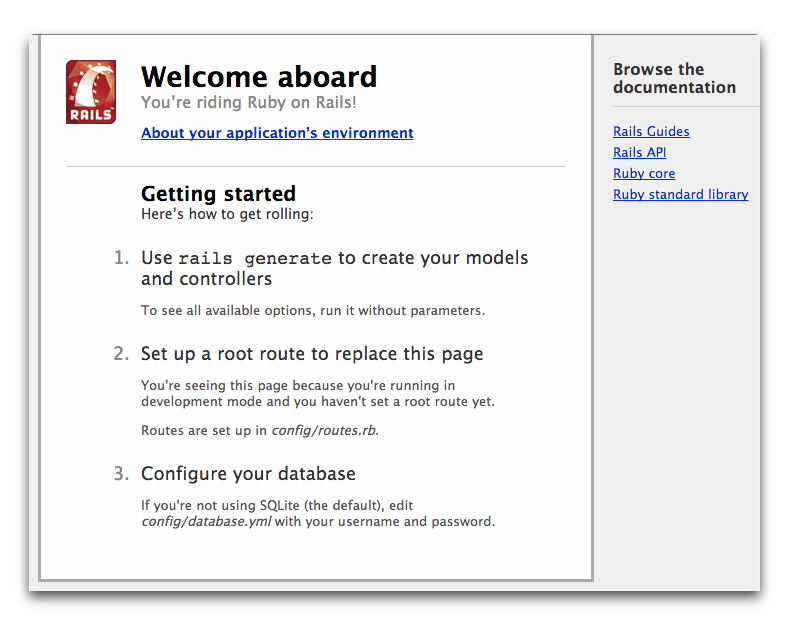
\includegraphics[width=12cm]{./image/rails/rails_welcome.png}
	\end{center}
\end{figure}

La página de ``Welcome aboard'' es un test para una nueva aplicación de \textit{Rails}. Con ello se asegura que \textit{Ruby on Rails} ha sido configurado de forma correcta. También se puede acceder al link ``About your application's environment'' para ver un resumen del entorno de la aplicación.

Para detener el servidor web, hay que presionar las teclas Ctrl+C en la ventana del terminal en la que el servidor web está siendo ejecutado.

\section{Modelos}
Como se ha dicho varias veces, \textit{Rails} usa el patrón de arquitectura MVC. Los modelos son la capa o parte del sistema responsable de representar la lógica de negocio. Los modelos de \textit{Rails} son diseñados y representados mediante Active Record.

\subsection{Active Record}
Active Record facilita la creación y uso de los objetos negocio cuyos datos precisan de ser persistentes en la base de datos.

Active Record es un objeto que envuelve una fila de una tabla o vista de una base de datos, encapsula el acceso a la base de datos, y añade lógica de negocio en esos datos envueltos. Active Record conlleva tanto tantos como comportamiento y muchos de estos datos deben de ser persistentes en la base de datos. Active Record añade acceso lógico a los datos en el dominio del objeto, de esta manera, todo el mundo sabe como leer y escribir los datos en la base de datos. \cite{Fowler2002}

Active Record es una descripción de ORM (Object-Relational-Mapping), que es una tecnica que conecta objetos de la aplicación con las tables de una base de datos relacional. Usando ORM, las propiedades de las relaciones de los objetos en una aplicación pueden ser facilmente almacenados y recuperados desde la base de datos, sin escribir consultas SQL directamente.

Active Record proporciona varios mecanismos propios de una técnica ORM:

\begin{enumerate}
	\item Representar modelos y sus datos.
	\item Representar asociaciones entre los modelos.
	\item Representar jerarquías de herencia a través de los modelos relacionados.
	\item Validar modelos antes de ser escritos de forma persistente a la base de datos.
	\item Realizar operaciones en la base de datos con una sintaxis y un estilo de orientación a objetos.
\end{enumerate}

\subsection{Convención sobre configuración en Active Record}
A diferencia de otros lenguajes de programación o frameworks, en \textit{Rails} no es necesario escribir mucha configuración cuando se trabaja con modelos de Active Record.

Por defecto, Active Record utiliza convenciones en los nombres para entender como un modelo y la la tabla de la base de datos deberían ser creados. \textit{Rails} pluraliza los nombres de las clases para encontrar la respectiva tabla de la base de datos. \footnote{La pluralización de \textit{Rails} es muy potente, siendo capaz de pluralizar o singularizar palabras regulares e irregulares.}

Active Record también utiliza convenciones para los nombres de las columnas de la base de datos, dependiendo del propósito de las columnas. 

\begin{description}
	\item[Claves ajenas] Los campos deben ser llamamos siguiendo el patrón nombre de la tabla singularizado e id. Por ejemplo, \texttt{user\_id} de la tabla \texttt{users}.
	\item[Claves primarias] Por defecto, Active Record utilizará una columna de tipo en tero llamada \texttt{id} como clave primaria.
\end{description}

\subsection{Creando modelos Active Record}

Para crear modelos de Active Record, lo único que se precisa hacer es asignarlo como subclase de \texttt{ActiveRecord::Base}

\begin{lstlisting}[language=Ruby]
class Product < ActiveRecord::Base
end
\end{lstlisting}

Esto permite crear un modelo \texttt{Product} que será referenciado a la tabla \texttt{products} de la base de datos. De esta manera, se posibilita la forma de referenciar columnas de cada fila de la tabla de la base de datos con los atributos de las instancias del modelo.


Suponiendo que la tabla productos ha sido creada utilizando la siguiente sentencia SQL,

\begin{lstlisting}[language=SQL]
CREATE TABLE products (
   id int(11) NOT NULL auto_increment,
   name varchar(255),
   PRIMARY KEY  (id)
);
\end{lstlisting}

Será posible escribir código como el siguiente:

\begin{lstlisting}[language=Ruby]
p = Product.new
p.name = "El Quijote"
puts p.name # "El Quijote"
\end{lstlisting}

\subsection{CRUD}
En computación CRUD es el acronimo de los cuatro verbos que usamos para operar con datos: Create, Read, Update y Delete. Active Record automaticamente crea estos métodos para permitir a la aplicación leer y manipular los datos almacenados en sus tablas.

\subsubsection{Create}
Los objetos de Active Record pueden ser creados desde un hash o manualmente establecidos después de su creación. El método \texttt{new} devuelve un objeto nuevo mientras que \texttt{create} retornará el objeto y lo almacenará en la base de datos.

El siguiente fragmento de código utiliza el método \texttt{create} por lo que creará el usuario y lo guardará como un nuevo registro en la base de datos.
\begin{lstlisting}[language=Ruby]
user = User.create(name: "Antonio", occupation: "Profesor")
\end{lstlisting}

Por el contrario, en este otro fragmento de código el usuario es creado pero no es guardado en la base de datos. 
\begin{lstlisting}[language=Ruby]
user = User.new
user.name = "Antonio"
user.occupation = "Profesor"
\end{lstlisting}

Si además se deseara guardar el usuario, se deberá utilizar el método \texttt{user.save}.

\subsubsection{Read}
Active Record proporciona una API potente para acceder a datos de la base de datos. A continuación se exponen una serie de ejemplos que ilustran los diferentes métodos facilitados por Active Record.


\begin{lstlisting}[language=Ruby]
# Devuelve una colección con todos los usuarios. 
users = User.all
\end{lstlisting}
 
\begin{lstlisting}[language=Ruby]
# Devuelve el primer usuario.
user = User.first 
\end{lstlisting}
 
\begin{lstlisting}[language=Ruby]
# Retorna el primer usuario con nombre Antonio
david = User.find_by(name: 'Antonio')  
\end{lstlisting}
  
\begin{lstlisting}[language=Ruby]
#Encuentra todos los usuarios llamados Antonio que son profesores ordenados por fecha de creación de forma inversa.
users = User.where(name: 'Antonio', occupation: 'Profesor').order(created_at: :desc)   
\end{lstlisting}

\subsubsection{Update}
Una vez que un objeto de Active Record ha sido recuperado, sus atributos pueden ser modificados y pueden ser guardados en la base de datos.

\begin{lstlisting}[language=Ruby]
user = User.find_by(name: 'David')
user.name = 'Antonio'
user.save
\end{lstlisting}

\begin{lstlisting}[language=Ruby]
# Otra forma de realizarlo
user = User.find_by(name: 'David')
user.update(name: 'Antonio')
\end{lstlisting}

\subsubsection{Delete}
Análogamente, un objeto de Active Record recuperado puede ser destruido, lo que le borra de la base de datos.

\begin{lstlisting}[language=Ruby]
user = User.find_by(name: 'Antonio')
user.destroy
\end{lstlisting}


\subsection{Migraciones de la base de datos}
Las migraciones de \textit{Rails} son la forma mas conveniente de alterar el esquema de la base de datos de una manera consistente y sencilla. Las migraciones usan un Ruby DSL (Domain Specific Language) por lo que no hace falta escribir ni una sola instrucción SQL, permitiendo que el esquema de la base de datos y los cambios ser independientes de la base de datos.

Se puede pensar que una migración es una nueva ``versión'' de la base de datos. Active Record actualiza el archivo \texttt{db/schema.rb} para mantener la estructura actualizada de la base de datos.

Un ejemplo de una migración:

\begin{lstlisting}[language=Ruby]
class CreateProducts < ActiveRecord::Migration
  def change
    create_table :products do |t|
      t.string :name
      t.text :description
 
      t.timestamps null: false
    end
  end
end
\end{lstlisting}

Las migraciones pueden ser lanzadas hacia ``delante'' o hacia ``detrás'', esto significa que si, por ejemplo, la migración anterior es lanzada cuando no existe la tabla \texttt{products} en la base de datos, entonces, la tabla \texttt{products} con las columnas \texttt{name}, \texttt{descripción}, y \texttt{timestamps} será creada. Por el contrario, si lanzamos la migración cuando la tabla existe en la base de datos, lo que se producirá es un efecto de \textit{rollback}.

En las bases de datos que soportan transacciones con instrucciones que modifiquen el esquema, las migraciones son envueltas en una transacción, de forma que si una migración falla, se hará un \textit{rollback} automáticamente de la transacción.\footnote{Si la base de datos no soporta transacciones y la migración falla, los cambios para hacer el rollback deben ser realizados manualmente.}

Algunas migraciones contienen ciertas instrucciones que Active Record no sabe como hacer el inverso de dicha operación. El ejemplo más típico es el cambio de nombre.

\begin{lstlisting}[language=Ruby]
class ChangeProductsPrice < ActiveRecord::Migration
  def up
    change_table :products do |t|
      t.change :price, :string
    end
  end
 
  def down
    change_table :products do |t|
      t.change :price, :integer
    end
  end
end
\end{lstlisting}


\subsubsection{Creando una migración simple}
Las migraciones son almacenadas en ficheros en el directorio \texttt{db/migrate}, un fichero por cada migración. El nombre del fichero contiene el UTC timestamp que es la fecha en formato YYYYMMDDHHMMSS (año, mes, día, hora, minuto, segundo) seguido de guión bajo y el nombre de la migración. \textit{Rails} usa el UTC timestamp para determinar el orden en el que las migraciones deben ser ejecutadas.

Se puede generar una migración de la siguiente forma:

\begin{lstlisting}[language=bash]
$ bin/rails generate migration AddPartNumberToProducts
\end{lstlisting}

Ese comando creará un nuevo archivo en \texttt{db/migrate} que contendrá:

\begin{lstlisting}[language=Ruby]
class AddPartNumberToProducts < ActiveRecord::Migration
  def change
  end
end
\end{lstlisting}

Si el nombre de la migración sigue el patrón AddXXXToYYY o RemoveXXXFromYYY seguido de una lista de nombres de columnas y sus tipos, entonces la migración será creada con las instrucciones \texttt{add\_column} y \texttt{remove\_column}, respectivamente.

\begin{lstlisting}[language=bash]
$ bin/rails generate migration AddPartNumberToProducts part_number:string
\end{lstlisting}

\begin{lstlisting}[language=Ruby]
lass AddPartNumberToProducts < ActiveRecord::Migration
  def change
    add_column :products, :part\_number, :string
  end
end
\end{lstlisting}


\myparagraph{Generadores de Modelos}
El modelo y los \textit{scaffold generators} crean las migraciones apropiadas para el nuevo modelo. Esta migración contendrá instrucciones para crear la tabla de la base de datos. 

\begin{lstlisting}[language=bash]
$ bin/rails generate model Product name:string description:text 
\end{lstlisting}  

El generador anterior creará el nuevo modelo y una migración nueva con el siguiente contenido:

\begin{lstlisting}[language=Ruby]
class CreateProducts < ActiveRecord::Migration
  def change
    create_table :products do |t|
      t.string :name
      t.text :description
 
      t.timestamps null: false
    end
  end
end
\end{lstlisting}


\subsubsection{Sintaxis de las migraciones}

\myparagraph{Tablas}
El método \texttt{create\_table} es el más fundamental y casi siempre es creado por un generador de modelos o un \textit{scaffold generator}. Implícitamente crea una columna \texttt{id} que será la clave primaria.

\begin{lstlisting}[language=Ruby]
create_table :products do |t|
  t.string :name
end
\end{lstlisting}

\myparagraph{Join Table}
El método de migración \texttt{create\_join\_table} crea una tabla join para una relación de muchos a muchos o HABTM.\footnote{Has and belongs to many}

\begin{lstlisting}[language=Ruby]
create_join_table :products, :categories
\end{lstlisting}

\begin{lstlisting}[language=Ruby]
create_join_table :products, :categories do |t|
  t.index :product_id
  t.index :category_id
end
\end{lstlisting}


\myparagraph{Modificación de columnas}
Los métodos de modificación de columnas son los siguientes:

\begin{lstlisting}[language=Ruby]
change_column :products, :part_number, :text
\end{lstlisting}

\begin{lstlisting}[language=Ruby]
add_column :products, :description, :string
\end{lstlisting}

\begin{lstlisting}[language=Ruby]
remove_column :products, :description
\end{lstlisting}

\subparagraph{Modificadores de columnas}
Los modificadores de columnas pueden aplicados cuando se crea o se modifica una columna.

\begin{description}
	\item[\texttt{limit}] Establece el tamaño máximo de los campos de tipo \texttt{string / text / binary / integer}
	\item[\texttt{precision}] Define la precisión para los campos de tipo \texttt{decimal}, representando el numero total de dígitos en el número.
	\item[\texttt{scale}] Define la escala para los campos de tipo \texttt{decimal}, representando el número de dígitos después del punto decimal. 
	\item[\texttt{polymorphic}] Este parámentro añade una columna del tipo \texttt{type} para las asociaciones \texttt{belongs\_to}.
	\item[\texttt{null}] Habilita o inhabilita valores de tipo \texttt{NULL} en la columna.
	\item[\texttt{default}] Permite establecer un valor por defecto en la columna.
	\item[\texttt{index}] Añade un índice a la columna.
	\item[\texttt{required}] Añade \texttt{required: true} para las asociaciones \texttt{belongs\_to} y \texttt{null: false} a la columna en la migración.
\end{description}

\myparagraph{Claves ajenas}
Las claves ajenas ayudan a mantener la integridad referencial de una base de datos.

\begin{lstlisting}[language=Ruby]
add_foreign_key :articles, :authors
\end{lstlisting}

Añade la clave ajena, introduciendo la columna \texttt{author\_id} en la tabla \texttt{articles}. La clave referencia a la columna \texttt{id} en la tabla \texttt{authors}.

Active Record solo soporta claves ajenas de una sola columna. Para claves ajenas compuestas se precisa \texttt{execute} y \texttt{structure.sql}.

Hay varias opciones para eliminar claves ajenas:

\begin{lstlisting}[language=Ruby]
# Active Record buscará el nombre de columna.
remove_foreign_key :accounts, :branches

#Elimina la clave ajena de una columna especifica.
remove_foreign_key :accounts, column: :owner_id
 
# Elimina la clave ajena por su nombre.
remove_foreign_key :accounts, name: :special_fk_name
\end{lstlisting}

\myparagraph{Ejecutar SQL}
Si Active Record no fuera suficiente, se pueden ejecutar instrucciones directamente en lenguaje SQL mediante el método \texttt{execute}.\footnote{Documentación relacionada en la API de \textit{Ruby on Rails}, \url{http://api.rubyonrails.org/classes/ActiveRecord/ConnectionAdapters/SchemaStatements.html}}

\begin{lstlisting}[language=Ruby]
Product.connection.execute('UPDATE `products` SET `price`=`free` WHERE 1')
\end{lstlisting}

\myparagraph{Rollback}
Como se ha mencionado anteriormente, \textit{Rails} soporta rollbacks de las migraciones a la base de datos, porporcionando diversos métodos:

\subparagraph{Método \texttt{change}}
El método \texttt{change} es el método primario y por defecto de las migraciones. Funciona en la mayoría de los casos que son aquellos en los cuales Active Record sabe cual es la migración inversa. El método \texttt{change} soporta las siguientes definiciones:

\begin{enumerate}
	\item add\_column
	\item add\_index
	\item add\_reference
	\item add\_timestamps
	\item add\_foreign\_key
	\item add\_table
	\item add\_join\_table
	\item drop\_table (si se proporciona un bloque con el contenido)
	\item drop\_join\_table (si se proporciona un bloque con el contenido)
	\item remove\_timestamps
	\item rename\_column
	\item rename\_index
	\item rename\_reference
	\item rename\_table
\end{enumerate}

\subparagraph{Método \texttt{reversible}}
Otros métodos o algunas migraciones complejas requieren procesado que Active Record no sabe como hacer la operación inversa. Para solucionarlo, el método \texttt{reversible} permite especificar que se debe de hacer cuando se ejecuta una migración y cuando se revierte una migración.

\begin{lstlisting}[language=Ruby]
class ExampleMigration < ActiveRecord::Migration
  def change
    create_table :distributors do |t|
      t.string :zipcode
    end
 
    reversible do |dir|
      dir.up do
        # add a CHECK constraint
        execute <<-SQL
          ALTER TABLE distributors
            ADD CONSTRAINT zipchk
              CHECK (char_length(zipcode) = 5) NO INHERIT;
        SQL
      end
      dir.down do
        execute <<-SQL
          ALTER TABLE distributors
            DROP CONSTRAINT zipchk
        SQL
      end
    end
 
    add_column :users, :home_page_url, :string
    rename_column :users, :email, :email_address
  end
end
\end{lstlisting}

En lo casos en los que una migración sea totalmente irreversible, como cuando se destruyen algunos datos, se puede lanzar una excepción de \texttt{ActiveRecord::IrreversibleMigration} en el bloque \texttt{down}, de forma que si alguien intenta realizar la migración, un mensaje de error será emitido.

\subparagraph{Método \texttt{up/down}}

Además de el método reversible, existe el método \texttt{up/down} que similar funcionalmente pero la sintaxis es distinta.

\begin{lstlisting}[language=Ruby]
class ExampleMigration < ActiveRecord::Migration
  def up
    create_table :distributors do |t|
      t.string :zipcode
    end
 
    # add a CHECK constraint
    execute <<-SQL
      ALTER TABLE distributors
        ADD CONSTRAINT zipchk
        CHECK (char_length(zipcode) = 5);
    SQL
 
    add_column :users, :home_page_url, :string
    rename_column :users, :email, :email_address
  end
 
  def down
    rename_column :users, :email_address, :email
    remove_column :users, :home_page_url
 
    execute <<-SQL
      ALTER TABLE distributors
        DROP CONSTRAINT zipchk
    SQL
 
    drop_table :distributors
  end
end
\end{lstlisting}


\subsubsection{Ejecución de migraciones}
\textit{Rails} proporciona un conjunto de tareas Rake para ejecutar migraciones.
La migración sencilla ejecuta el método \texttt{change} o el método \texttt{up} para todas las migraciones que aún no han sido ejecutadas. Si no hay migraciones, estas se ejecutarán en base al orden de creación de su UTC timestamp. 

\begin{lstlisting}[language=bash]
$ bin/rake db:migrate
\end{lstlisting}

Si se especifica una versión, Active Record ejecutará las migraciones requeridas (\texttt{change}, \texttt{up}, \texttt{down}) hasta que se alcance la versión especificada.

\begin{lstlisting}[language=bash]
$ bin/rake db:migrate VERSION=20150906120000
\end{lstlisting}

\myparagraph{Rollback}
Un rollback habitual es volver a la migración anterior debido a un error, por ejemplo.

\begin{lstlisting}[language=bash]
$ bin/rake db:rollback
\end{lstlisting}

Mediante el parámetro \texttt{STEP}, especificamos cuantas migraciones se deben revertir.

\begin{lstlisting}[language=bash]
$ bin/rake db:rollback STEP=3
\end{lstlisting}

Si se desea revertir una o varias migraciones y luego migrar otra vez, existe un atajo:

\begin{lstlisting}[language=bash]
$ bin/rake db:migrate:redo STEP=3
\end{lstlisting}

Por último, y como consecuencia lógica de la funcionalidad cuando se especifica una version concreta, si se pretende revertir hasta cierto punto o momento, se debe especificar con el parámetro \texttt{VERSION}.

\begin{lstlisting}[language=bash]
$ bin/rake db:migrate VERSION=20150906120000
\end{lstlisting}

\myparagraph{Otras tareas Rake}
Otras tareas y operaciones con Rake frecuentes son las siguientes:

\begin{description}
	\item[\texttt{rake db:setup}] Esta tarea crea la base de datos, carga el esquema y la inicializa con los datos semilla.
	\item[\texttt{rake db:drop}] Esta operación destruye la base de datos y el esquema.
	\item[\texttt{rake db:reset}] Esta operación es similar a realizar \texttt{rake db:drop} y después \texttt{rake db:setup}.\footnote{Esta operación no es lo mismo que ejecutar todas las migraciones. Sólo usará los contenidos del archivo \texttt{schema.rb} actual. Si una migración no puede ser revertida, \texttt{rake db:reset} no será útil probablemente.} 
\end{description}

Por defecto, \texttt{rake db:migrate} es una instrucción que siempre se ejecutará en modo desarrollo (\texttt{development}). Si se desea ejecutar migraciones en otro entorno que no sea el de desarrollo se puede especificar usando la variable \texttt{RAILS\_ENV} mientras se ejecuta el comando.

\begin{lstlisting}[language=bash]
$ bin/rake db:migrate RAILS_ENV=test
\end{lstlisting}

\begin{lstlisting}[language=bash]
$ bin/rake db:rollback RAILS_ENV=production
\end{lstlisting}

\myparagraph{Migraciones y datos semilla}
Se pueden usar migraciones para añadir datos a la base de datos:

\begin{lstlisting}[language=Ruby]
class AddInitialProducts < ActiveRecord::Migration
  def up
    5.times do |i|
      Product.create(name: "Product ##{i}", description: "A product.")
    end
  end
 
  def down
    Product.delete_all
  end
end
\end{lstlisting}

Sin embargo, \textit{Rails} tiene una funcionalidad de semillas que será usada para poblar bases de datos. Se trata añadir código al archivo \texttt{db/seeds.rb} y después, ejecuta el comando \texttt{rake db:seed}.

\begin{lstlisting}[language=Ruby]
5.times do |i|
  Product.create(name: "Product ##{i}", description: "A product.")
end
\end{lstlisting} 


\subsection{Validaciones}
\subsubsection{Introducción}

Validación es el proceso que garantiza que un dato o conjunto de datos cumple con los requisitos y especificaciones necesarias para ser introducido en el sistema de forma persistente.

\begin{lstlisting}[language=Ruby]
class Person < ActiveRecord::Base
  validates :name, presence: true
end
 
Person.create(name: "Thomas A. Anderson").valid? # => true
Person.create(name: nil).valid? # => false
\end{lstlisting}
 
Las validaciones a nivel de modelo son la mejor forma en \textit{Rails} para asegurar que los datos datos que se guardan en la base de datos son correctos.
Además de validar los datos a nivel de modelo, existen otras formas de validar los datos:

\begin{enumerate}
	\item Restricciones y procedimientos almacenados que hacen la validación dependiente de la base de datos por lo que el testeo y el mantenimiento es más complicado. Sin embargo, si la base de datos es utilizada por otras aplicaciones, es ventajoso poner las restricciones a nivel de la base de datos.
	\item Las validaciones en el cliente pueden ser útiles pero no fiables si se usan por si mismas.
	\item Las validaciones al nivel del controlador son difíciles de testear y mantener. Siguiendo una de las filosofias de \textit{Ruby on Rails}, lso controladores deben ser simples en cuanto a complejidad mientras que los modelos deben complejos.
\end{enumerate}

Hay muchas formas de cambiar los estados de los objetos en la base de datos. Algunos métodos implican la ejecución de disparadores de validación, pero otros no. Por tanto, es posible guardar un objeto inválido en la base de datos si no se trata con cuidado.

Los siguientes métodos lanzan validaciones. La diferencia es que los que tienen exclamación lanzan una excepción si el objeto es inválido mientras que los otros retornan false (\texttt{save} y \texttt{update}) o el objeto (\texttt{create}).
 
\begin{enumerate}
	\item \texttt{create}
	\item \texttt{create!}
	\item \texttt{save}
	\item \texttt{save!}
	\item \texttt{update}
	\item \texttt{update!}
\end{enumerate}

Los siguientes métodos saltan las validaciones, y por tanto, guardarán el objeto en la base de dato independientemente de su validez:

\begin{enumerate}
	\item \texttt{decrement!}
	\item \texttt{decrement\_counter}
	\item \texttt{increment!}
	\item \texttt{increment\_counter}
	\item \texttt{toggle!}
	\item \texttt{update\_all}
	\item \texttt{update\_attribute}
	\item \texttt{update\_column}
	\item \texttt{update\_columns}
	\item \texttt{update\_counters}
	\item Además \texttt{save} también tiene la habilidad de saltar validaciones si utiliza con el argumento \texttt{validate: false}.
\end{enumerate}

Para verificar si un objeto es válido o inválido, \textit{Rails} usa el método \texttt{valid?}.

\begin{lstlisting}[language=Ruby]
class Person < ActiveRecord::Base
  validates :name, presence: true
end
 
Person.create(name: "Thomas A. Anderson").valid? # => true
Person.create(name: nil).valid? # => false
\end{lstlisting}

Un objeto instanciado con el método \texttt{new} no reportará errores de validación incluso si es inválido debido a que las validaciones no son disparadas cuando se utiliza el método \texttt{new}.

\begin{lstlisting}[language=Ruby]
class Person < ActiveRecord::Base
  validates :name, presence: true
end
 
>> p = Person.new
# => #<Person id: nil, name: nil>
>> p.errors.messages
# => {}
 
>> p.valid?
# => false
>> p.errors.messages
# => {name:["can't be blank"]}
 
>> p = Person.create
# => #<Person id: nil, name: nil>
>> p.errors.messages
# => {name:["can't be blank"]}
 
>> p.save
# => false
 
>> p.save!
# => ActiveRecord::RecordInvalid: Validation failed: Name can't be blank
 
>> Person.create!
# => ActiveRecord::RecordInvalid: Validation failed: Name can't be blank
\end{lstlisting}

Para verificar si un atributo en particular de un objeto es válido, se puede utilizar el método \texttt{errors[:attribute]}. El método retorna un vector con todos los errores del atributo \texttt{:attribute}. Si no hay errores en dicho atributo, un array vació será retornado.

\begin{lstlisting}[language=Ruby]
class Person < ActiveRecord::Base
  validates :name, presence: true
end
 
>> Person.new.errors[:name].any? # => false
>> Person.create.errors[:name].any? # => true
\end{lstlisting}


\subsubsection{Procedimientos de validación}

Active Record proporciona un conjunto de procedimientos de validación que pueden ser directamente usados en las clases. Estos procedimientos proporcionan reglas comunes de validación. Siempre que una validación falla, un mensaje de error es añadido a la colección de errores del objeto con un mensaje asociado al atributo validado.

\myparagraph{\texttt{acceptance}}
Éste método valida que una checkbox en el interfaz de usuario ha sido seleccionada cuando el formulario ha sido enviado. El mensaje de error por defecto es ``must be accepted''.

\begin{lstlisting}[language=Ruby]
class Person < ActiveRecord::Base
  validates :terms_of_service, acceptance: true
end
\end{lstlisting}

\myparagraph{\texttt{validates\_associated}}
El método \texttt{validates\_associated} debe ser utilizado cuando el modelo tiene asociaciones con otros modelos que también necesitan ser validados.\footnote{Es importante no utilizar el método \texttt{validates\_associated} en ambos extremos de la asociación, puesto que se llamarán unos a otros creando un bucle infinito.} El mensaje de error por defecto del método es ``is invalid''.

\begin{lstlisting}[language=Ruby]
class Library < ActiveRecord::Base
  has_many :books
  validates_associated :books
end
\end{lstlisting}

\myparagraph{\texttt{confirmation}}
Éste procedimiento se puede utilizar cuando dos campos de texto reciben exactamente el mismo contenido como en una validación de una contraseña. El mensaje de error por defecto es ``doesn't match confirmation''.

\begin{lstlisting}[language=Ruby]
#Modelo
class Person < ActiveRecord::Base
  validates :email, confirmation: true
end 

#Vista
<%= text_field :person, :email %>
<%= text_field :person, :email_confirmation %>
\end{lstlisting}


\myparagraph{\texttt{exclusion}}
El procedimiento \texttt{exclusion} valida que los valores de los atributos no estén incluidos en un conjunto dado. Éste método, además, incorpora una opción \texttt{:in} que recibe un conjunto de valores que no serán aceptados por el atributo al ser validado.\footnote{La opción \texttt{:in} posee un alias \texttt{:within} que realiza la misma funcionalidad.} El mensaje de error es ìs reserved''.

\begin{lstlisting}[language=Ruby]
class Account < ActiveRecord::Base
  validates :subdomain, exclusion: { in: %w(www us ca jp),
    message: "%{value} is reserved." }
end
\end{lstlisting}

\myparagraph{\texttt{format}}
El método \texttt{format} valida los valores de los atributos probando si coinciden o no con una expresión regular dada con la opción \texttt{:with} o \texttt{:without}, respectivamente. Por defecto, su mensaje de error es ``is invalid''.

\begin{lstlisting}[language=Ruby]
class Product < ActiveRecord::Base
  validates :legacy_code, format: { with: /\A[a-zA-Z]+\z/,
    message: "only allows letters" }
end
\end{lstlisting}

\myparagraph{\texttt{inclusion}}
Éste procedimiento es inverso al método \texttt{exclusion} y por tanto, valida que los valores de los atributos son incluidos en un conjunto dado. De la misma manera que \texttt{exclusion}, éste método posee las opciones \texttt{:in} o \texttt{:within}.

\begin{lstlisting}[language=Ruby]
class Coffee < ActiveRecord::Base
  validates :size, inclusion: { in: %w(small medium large),
    message: "%{value} is not a valid size" }
end
\end{lstlisting}

\myparagraph{\texttt{length}}
El método \texttt{length} valida que los valores de los atributos tengan una longitud concreta. Provee una serie de opciones, por lo que se puede especificar constantes de longitud de diversas formas.

\begin{description}
	\item[\texttt{:minumum}] El atributo no puede ser menor que la longitud especificada.
	\item[\texttt{:maximum}] El atributo no puede ser mayor que la longitud especificada.
	\item[\texttt{:in} o \texttt{:within}] El atributo debe estar incluido en el rango de la longitud especificada.
	\item[\texttt{:is}] El atributo deber ser igual que la longitud especificada.
\end{description}

\begin{lstlisting}[language=Ruby]
class Essay < ActiveRecord::Base
  validates :content, length: {
    minimum: 300,
    maximum: 400,
    tokenizer: lambda { |str| str.split(/\s+/) },
    too_short: "must have at least %{count} words",
    too_long: "must have at most %{count} words"
  }
end
\end{lstlisting}


\myparagraph{\texttt{numericality}}
El procedimiento valida que los atributos solo contengan valores numéricos. Por defecto, acepta cualquier valor numérico pero puede ser restringido a sólo enteros o flotantes. El error por defecto es ``is not a number''.

\begin{description}
	\item[\texttt{:greater\_than}] Especifica que el valor deber ser mayor que el valor proporcionado.
	\item[\texttt{:greater\_than\_or\_equal\_to}] Especifica que el valor deber ser mayor o igual que el valor proporcionado.
	\item[\texttt{:equal\_to}] Especifica que el valor deber ser igual que el valor proporcionado.
	\item[\texttt{:less\_than}] Especifica que el valor deber ser menor que el valor proporcionado.
	\item[\texttt{:less\_than\_or\_equal\_to}] Especifica que el valor deber ser menor o igual que el valor proporcionado.
	\item[\texttt{:odd}] Especifica que el valor debe ser impar.
	\item[\texttt{:even}] Especifica que el valor debe ser par.
\end{description} 

\myparagraph{\texttt{presence}}
Éste método valida que los atributos especificados con él no son vacíos.

\begin{lstlisting}[language=Ruby]
class Person < ActiveRecord::Base
  validates :name, :login, :email, presence: true
end
\end{lstlisting}

También puede ser utilizado para asegurar que una asociación es presente.

\begin{lstlisting}[language=Ruby]
class LineItem < ActiveRecord::Base
  belongs_to :order
  validates :order, presence: true
end

class Order < ActiveRecord::Base
  has_many :line_items, inverse_of: :order
end
\end{lstlisting}

\myparagraph{\texttt{absence}}
De forma contraria al método \texttt{presence}, éste procedimiento asegura los atributos especificados no son presentes.

\begin{lstlisting}[language=Ruby]
class Person < ActiveRecord::Base
  validates :name, :login, :email, absence: true
end
\end{lstlisting}

Analogamente al procedimiento \texttt{presence}, también puede ser utilizado para asegurar asociaciones.

\begin{lstlisting}[language=Ruby]
class LineItem < ActiveRecord::Base
  belongs_to :order
  validates :order, absence: true
end

class Order < ActiveRecord::Base
  has_many :line_items, inverse_of: :order
end
\end{lstlisting}

\myparagraph{\texttt{uniqueness}}
El procedimiento \texttt{uniqueness} valida que los valores de atributo son únicos antes de que el objeto sea guardado en la base de datos. El mensaje de error por defecto es ``has already been taken''. 

\begin{lstlisting}[language=Ruby]
class Account < ActiveRecord::Base
  validates :email, uniqueness: true
end
\end{lstlisting}

La opción \texttt{:scope} permite especificar otros atributos que son utilizados para limitar la validación

\begin{lstlisting}[language=Ruby]
class Holiday < ActiveRecord::Base
  validates :name, uniqueness: { scope: :year,
    message: "should happen once per year" }
end
\end{lstlisting}

La opción \texttt{:case\_sensitive} define si la unicidad debe ignorar mayúsculas y minúsculas.

\myparagraph{\texttt{validates\_with}}
Éste método pasa el registro a otra clase para emprender la validación.

\begin{lstlisting}[language=Ruby]
class GoodnessValidator < ActiveModel::Validator
  def validate(record)
    if record.first_name == "Evil"
      record.errors[:base] << "This person is evil"
    end
  end
end
 
class Person < ActiveRecord::Base
  validates_with GoodnessValidator
end
\end{lstlisting}


\subsubsection{Opciones de validación}

Las opciones de validación más comunes son:

\begin{description}
	\item[\texttt{:allow\_nil}] Salta la validación cuando el valor evaluado es \texttt{nil}.
\begin{lstlisting}[language=Ruby]
  class Coffee < ActiveRecord::Base
    validates :size, inclusion: { in: %w(small medium large),
      message: "%{value} is not a valid size" }, allow_nil: true
  end
\end{lstlisting}

	\item[\texttt{:allow\_blank}] Ésta opción ignora la validación si el valor es \texttt{nil} o una cadena de texto vacía.	
\begin{lstlisting}[language=Ruby]
class Topic < ActiveRecord::Base
  validates :title, length: { is: 5 }, allow_blank: true
end
 
Topic.create(title: "").valid?  # => true
Topic.create(title: nil).valid? # => true
\end{lstlisting}

	\item[\texttt{:message}] La opción \texttt{:message} permite especificar el mensaje que será añadido a la colección de errores cuando la validación falla.
	
	\item[\texttt{:on}] Permite especificar cuando la validación debe ocurrir.
	
\begin{lstlisting}[language=Ruby]
class Person < ActiveRecord::Base
  # it will be possible to update email with a duplicated value
  validates :email, uniqueness: true, on: :create
 
  # it will be possible to create the record with a non-numerical age
  validates :age, numericality: true, on: :update
 
  # the default (validates on both create and update)
  validates :name, presence: true
end	
\end{lstlisting}
	
\end{description}

\subsubsection{Validación condicional}
Se puede validar un objeto solamente cuando cierta condición es satisfecha. Para ello, \textit{Rails} habilita los métodos \texttt{:if} y \texttt{unless}.

\begin{description}
	\item[\texttt{Symbol} con \texttt{:if} y \texttt{:unless}] Se puede asociar \texttt{:if} y \texttt{:unless} con un símbolo que corresponde con el nombre un método que será llamado cuando la validación ocurre.

\begin{lstlisting}[language=Ruby]
class Order < ActiveRecord::Base
  validates :card_number, presence: true, if: :paid_with_card?
 
  def paid_with_card?
    payment_type == "card"
  end
end
\end{lstlisting}

	\item[Cadena de caracteres con \texttt{:if} y \texttt{:unless}] Es posible utilizar una cadena que será evaluada con el método \texttt{eval}. 

\begin{lstlisting}[language=Ruby]
class Person < ActiveRecord::Base
  validates :surname, presence: true, if: "name.nil?"
end
\end{lstlisting}

	\item[Proc con \texttt{:if} y \texttt{:unless}] También es posible asociar \texttt{:if} y \texttt{:unless} con un objeto de la clase \texttt{Proc} que se será llamado. 

\begin{lstlisting}[language=Ruby]
class Account < ActiveRecord::Base
  validates :password, confirmation: true,
    unless: Proc.new { |a| a.password.blank? }
end
\end{lstlisting}

\end{description}

\myparagraph{Agrupado y combinado de validaciones}
Resulta útil y clarificador poder combinar múltiples condiciones en una sola condición.

\begin{lstlisting}[language=Ruby]
class User < ActiveRecord::Base
  with_options if: :is_admin? do |admin|
    admin.validates :password, length: { minimum: 10 }
    admin.validates :email, presence: true
  end
end
\end{lstlisting}

De la misma manera se pueden combinar condiciones múltiples cuando una validación debe ocurrir o no.

\begin{lstlisting}[language=Ruby]
class Computer < ActiveRecord::Base
  validates :mouse, presence: true,
                    if: ["market.retail?", :desktop?],
                    unless: Proc.new { |c| c.trackpad.present? }
end
\end{lstlisting}

\subsubsection{Validaciones personalizadas}
Las validaciones personalizadas son creadas a través de clases que heredan de la clase \texttt{ActiveModel::Validator}. Éstas clases deben implementar un método \texttt{validate} que toma un argumento y le aplica la validación. Las validaciones personalizadas son ejecutadas llamando al método \texttt{validates\_with}.

\begin{lstlisting}[language=Ruby]
class MyValidator < ActiveModel::Validator
  def validate(record)
    unless record.name.starts_with? 'X'
      record.errors[:name] << 'Need a name starting with X please!'
    end
  end
end
 
class Person
  include ActiveModel::Validations
  validates_with MyValidator
end
\end{lstlisting}

También se pueden crear métodos personalizados que verifiquen el estado de los modelos y añadan mensajes a la colección de errores cuando son inválidos.

\begin{lstlisting}[language=Ruby]
class Invoice < ActiveRecord::Base
  validate :expiration_date_cannot_be_in_the_past,
    :discount_cannot_be_greater_than_total_value
 
  def expiration_date_cannot_be_in_the_past
    if expiration_date.present? && expiration_date < Date.today
      errors.add(:expiration_date, "can't be in the past")
    end
  end
 
  def discount_cannot_be_greater_than_total_value
    if discount > total_value
      errors.add(:discount, "can't be greater than total value")
    end
  end
end
\end{lstlisting}


\subsection{Callbacks}

Los \textit{callbacks} son métodos que son invocados en ciertos momentos de la vida de los objetos. Con ellos es posible escribir código que será ejecutado cuando un objeto Active Record es creado, guardado, actualizado, borrado, validado, o cargado de la base de datos.

\begin{lstlisting}[language=Ruby]
class User < ActiveRecord::Base
  validates :login, :email, presence: true
 
  before_validation :ensure_login_has_a_value
 
  protected
    def ensure_login_has_a_value
      if login.nil?
        self.login = email unless email.blank?
      end
    end
end
\end{lstlisting}



\myparagraph{Callbacks disponibles}
Los \textit{callbacks} de \textit{Rails} disponibles son los siguientes:

\begin{itemize}
	\item Creación del objeto
	\begin{itemize}
		\item \texttt{before\_validation}
		\item \texttt{after\_validation}
		\item \texttt{before\_save}
		\item \texttt{around\_save}
		\item \texttt{before\_create}
		\item \texttt{around\_create}
		\item \texttt{after\_create}
		\item \texttt{after\_save}
		\item \texttt{after\_commit} o \texttt{after\_rollback}
	\end{itemize}
	\item Actualización del objeto
	\begin{itemize}
		\item \texttt{before\_validation}
		\item \texttt{after\_validation}
		\item \texttt{before\_save}
		\item \texttt{around\_save}
		\item \texttt{before\_update}
		\item \texttt{around\_update}
		\item \texttt{after\_update}
		\item \texttt{after\_save}
		\item \texttt{after\_commit} o \texttt{after\_rollback} 
	\end{itemize}
	\item Destrucción del objeto
	\begin{itemize}
		\item \texttt{before\_destroy}
		\item \texttt{around\_destroy}
		\item \texttt{after\_destroy}
		\item \texttt{after\_commit} o \texttt{after\_rollback}
	\end{itemize}
	\item Otros \textit{callbacks}
	\begin{itemize}
		\item \texttt{after\_initialize} es un \textit{callback} que será invocado cuando el objeto de Active Record es instanciado, ya sea mediante el método \texttt{new} o cargado desde la base de datos.
		\item \texttt{after\_find} es un \textit{callback} llamado cuando un objeto Active Record es cargado desde la base de datos.
		\item \texttt{after\_touch} es un \textit{callback} invocado cada vez que un objeto de Active Record es tocado. 
	\end{itemize}		
\end{itemize}



\myparagraph{Ejecución de callbacks}
En \textit{Rails}, los métodos siguientes disparan \textit{callbacks}:

\begin{itemize}
	\item \texttt{create}
	\item \texttt{create!}
	\item \texttt{decrement!}
	\item \texttt{destroy}
	\item \texttt{destroy!}
	\item \texttt{destroy\_all}
	\item \texttt{increment!}
	\item \texttt{save}
	\item \texttt{save!}
	\item \texttt{save(validate: false)}
	\item \texttt{toggle!}
	\item \texttt{update\_attribute}
	\item \texttt{update}
	\item \texttt{update!}
	\item \texttt{valid?}
\end{itemize}

Adicionalmente, el \textit{callback} \texttt{after\_find} es disparado por los siguientes métodos de búsqueda.

\begin{itemize}
	\item \texttt{all}
	\item \texttt{first}
	\item \texttt{find}
	\item \texttt{find\_by}
	\item \texttt{find\_by\_*}
	\item \texttt{find\_by\_*!}
	\item \texttt{find\_by\_sql}
	\item \texttt{last}
\end{itemize}

\myparagraph{Callbacks relacionales}
Los \textit{callbacks} de \textit{Rails} pueden funcionar en relaciones de modelos, y pueden incluso ser definidas por las propias relaciones. Puede darse el caso de que cuando un objeto es destruido, también deberian ser destruidos los objetos que dependen del susodicho objeto.

\begin{lstlisting}[language=Ruby]
class User < ActiveRecord::Base
  has_many :articles, dependent: :destroy
end
 
class Article < ActiveRecord::Base
  after_destroy :log_destroy_action
 
  def log_destroy_action
    puts 'Article destroyed'
  end
end
 
>> user = User.first
=> #<User id: 1>
>> user.articles.create!
=> #<Article id: 1, user_id: 1>
>> user.destroy
Article destroyed
=> #<User id: 1>
\end{lstlisting}

\myparagraph{Callbacks condicionales}
De la misma forma que las validaciones, podemos ejecutar un \textit{callback} siempre y cuando se ejecute una condición concreta. Análogamente a las validaciones, los mecanismos empleados para los \textit{callbacks} condicionales son los mismos.

\begin{description}
	\item[\texttt{Symbol}] Las opciones \texttt{:if} y \texttt{:unless} pueden ser asociadas con un símbolo correspondiente al nombre de un método que será llamado antes de realizar el \textit{callback}.
\begin{lstlisting}[language=Ruby]
class Order < ActiveRecord::Base
  before_save :normalize_card_number, if: :paid_with_card?
end
\end{lstlisting}

	\item[Cadena de caracteres] Una cadena de caracteres de código \textit{Ruby} es admitida utilizando el método eval.
\begin{lstlisting}[language=Ruby]
class Order < ActiveRecord::Base
  before_save :normalize_card_number, if: "paid_with_card?"
end
\end{lstlisting}

	\item[\texttt{Proc}] \textit{Rails} posibilita la asociación a un objeto \texttt{Proc}.
\begin{lstlisting}[language=Ruby]
class Order < ActiveRecord::Base
  before_save :normalize_card_number,
    if: Proc.new { |order| order.paid_with_card? }
end
\end{lstlisting}

	\item[Callbacks con condiciones múltiples]
\begin{lstlisting}[language=Ruby]
class Comment < ActiveRecord::Base
  after_create :send_email_to_author, if: :author_wants_emails?,
    unless: Proc.new { |comment| comment.article.ignore_comments? }
end
\end{lstlisting}
\end{description}

\myparagraph{Clases callback}
\textit{Rails} permite crear clases que encapsulan métodos \textit{callback}, lo que facilita que otros modelos reutilicen esos \textit{callbacks}.

\begin{lstlisting}[language=Ruby]
class PictureFileCallbacks
  def after_destroy(picture_file)
    if File.exist?(picture_file.filepath)
      File.delete(picture_file.filepath)
    end
  end
end

class PictureFile < ActiveRecord::Base
  after_destroy PictureFileCallbacks.new
end
\end{lstlisting}

